% Prof. Dr. Ausberto S. Castro Vera
% UENF - CCT - LCMAT - Curso de Ci\^{e}ncia da Computa\c{c}\~{a}o
% Campos, RJ,  2022
% Disciplina: Paradigmas de Linguagens de Programa\c{c}\~{a}o
% Aluno: Ricardo Willian Pontes da Silva


\chapter{Ferramentas existentes e utilizadas}
Neste capítulo, serão apresentadas e demonstradas algumas ferramentas disponíveis para auxiliar no desenvolvimento utilizando a linguagem de programação Python. Serão abordados tópicos como: 
 \begin{itemize}
	\item Nome da ferramenta
	\item Versão atual e utilizada
	\item Descrição e informações
	\item Telas capturadas da ferramenta
	\item Endereço na Internet
\end{itemize}

    \section{Visual Studio Code}

O Visual Studio Code é um ambiente de desenvolvimento poderoso para a linguagem Python por meio dos seus recursos e cargas de trabalho de ciência de dados. Com a utilização do Visual Studio para a criação de códigos com a linguagem Python a aprendizagem se torna de fácil acesso e gratuita com diversas bibliotecas disponíveis no seu ambiente. Com a união dessas ferramentas, é possível criar aplicativos Web, serviços Web, aplicativos de desktop, scripts e computação científica no Visual Studio, podendo ser utilizados por cientistas e desenvolvedores profissionais e casuais.\\
  \begin{figure}[H]
	\begin{center}
		\caption{Ambiente de desenvolvimento no Visual Studio} \label{ling1}
		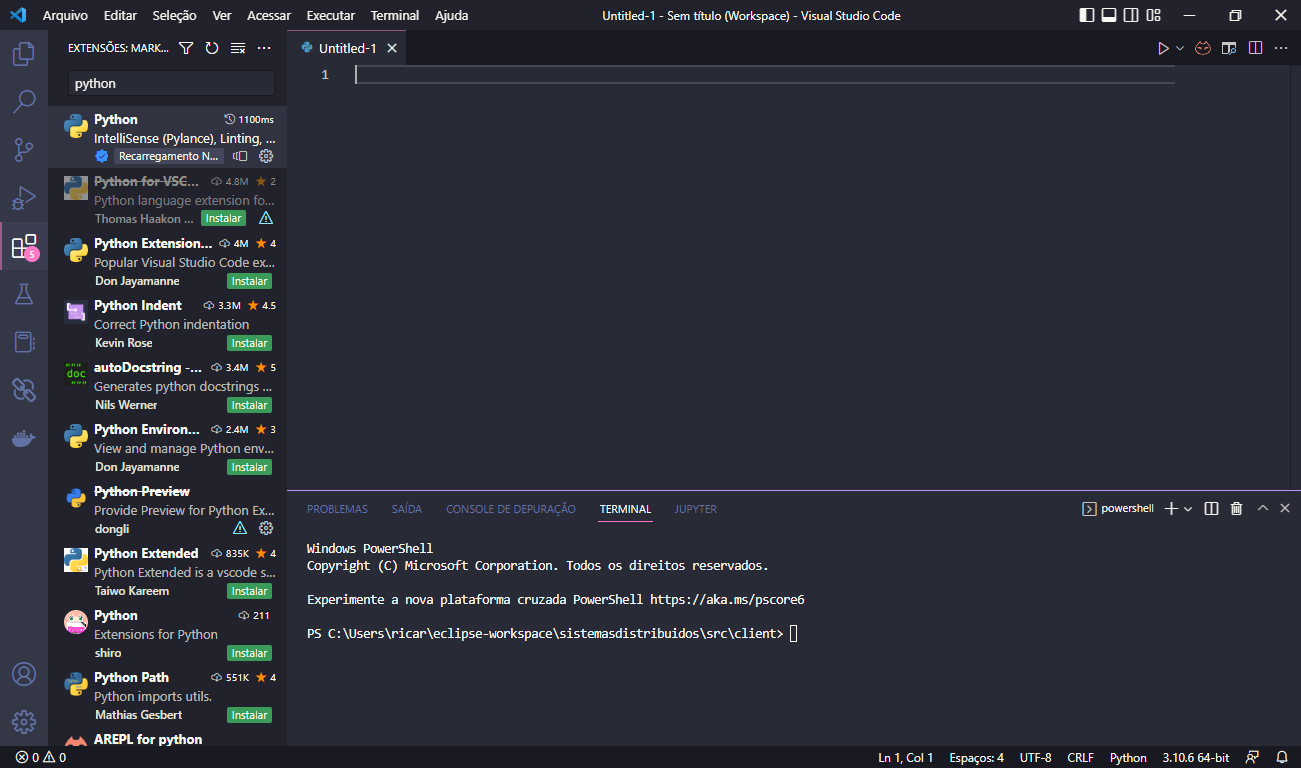
\includegraphics[width=15cm]{visualStudioPy.PNG} \\
		{\tiny \sf Fonte:{ Autor}}
	\end{center}
\end{figure}
A ferramenta Visual Studio é permissiva o desenvolvimento de N linguagens de programação e afins, desta forma, para utilizá-la para a linguagem Python é necessário selecionar e baixar no dispositivo as extensões necessárias para a mesma, como mostrado na figura acima. Atualmente o Visual Studio se encontra na versão 17.4 podendo ser utilizado também versões ainda em desenvolvimento e disponível para download em \href{https://visualstudio.microsoft.com/pt-br/downloads/}{Visual Studio Download}..

    \section{Compilador e interpretador CPython}

A implementação nativa do Python, CPython é o responsável pela operação da referência da linguagem Python, ou seja, o CPython compila a o código em Bytecode, e após, interpreta esse bytecode, executando-o. O CPython também se torna responsável pela sintaxe da linguagem, vale destacar também que o CPython permite a escrita de extensões C para o código Python. Ele também permite que você adicione a tipagem estática ao código Python existente, tornando-o compilado e obtendo desempenho semelhante ao C. Escrito na linguagem C e Python, o CPython é a principal implementação do Python atualmente utilizado, desta forma, para utiliza-lo basta baixar a versão mais recente do Python, que já consta com essa ferramenta. 


    \section{Ferramenta de controle e versionamento de código git} 
    Sistemas de controle de versões tem a capacidade de registrar as alterações feitas no código, armazenar essas informações e permitir que o programador volte para uma versão anterior do código, se necessário, de maneira fácil e rápida. Este tipo de sistema também simplifica muito o processo de compartilhamento de projetos com uma equipe ou outros programadores. Um dos mais famosos softwares de controle de versão na atualidade é o git, ao qual foi largamente utilizado para a realização do presente trabalho. É possível também fazer a união de IDE's como o Visual Studio Code já citado anteriormente com ferramentas do tipo git, para uma maior praticidade.
      \begin{figure}[H]
    	\begin{center}
    		\caption{Ferramentas git} \label{ling1}
    		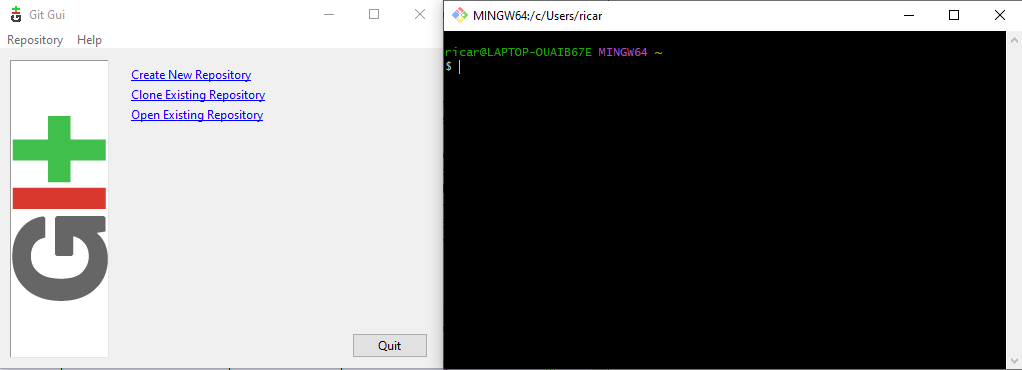
\includegraphics[width=15cm]{git.PNG} \\
    		{\tiny \sf Fonte:{ Autor}}
    	\end{center}
    \end{figure}
Atualmente é possível encontrar o git na versão 2.38.1 e disponível para download em \href{https://git-scm.com/download/win}{git Downloads}.